\begin{frame}[allowframebreaks,allowdisplaybreaks]
    \section{B-Tree}
    \subsection{History}
    \frametitle{B-Tree History}
    \begin{columns}
        \begin{column}{0.5\textwidth}
            \begin{block}{}
                B-Trees where firstly studied, defined and implemented by R. Bayer and E. McCreight in 1972, using an IBM 360 series model 44 with an 2311 disk drive.
                \begin{figure}
                    \centering
                    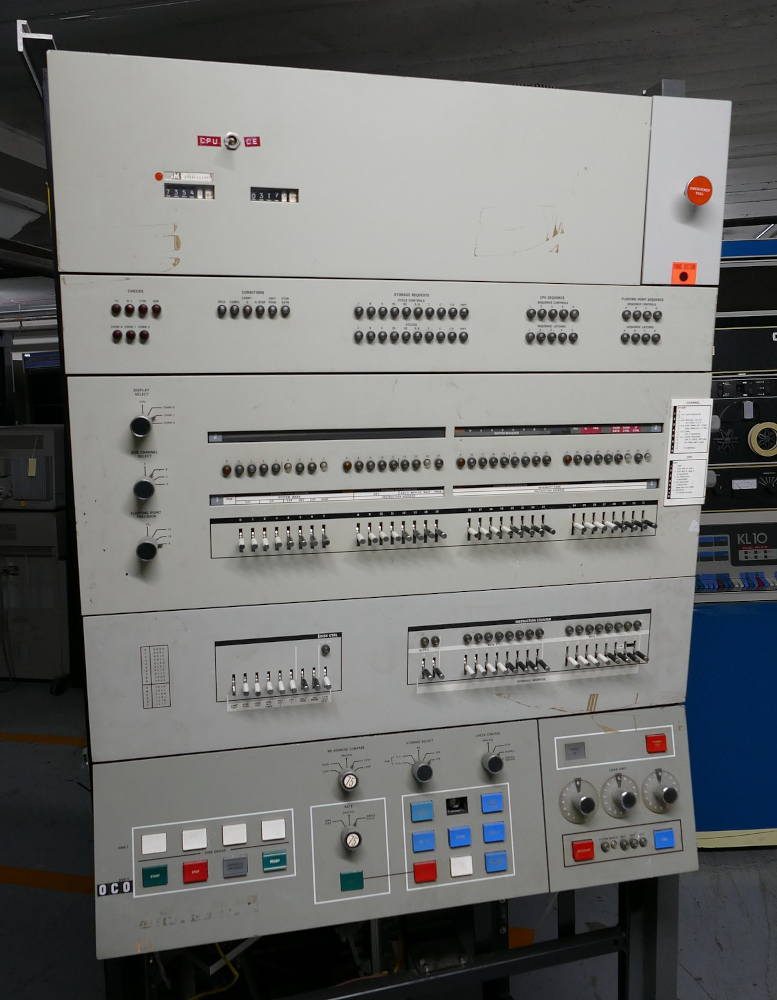
\includegraphics[width=0.5\textwidth,height=\textheight,keepaspectratio]{resources/made/ibm360_44.png}
                    \caption[]{IBM 360 / 44}
                \end{figure}
            \end{block}
        \end{column}
        \begin{column}{0.5\textwidth}
            \begin{block}{}
                An IBM 360 series model 44 had from 32 to 256 \(KB\) of Random Access Memory, and weighed from 1,315 to 1,905 kg.
                \begin{figure}
                    \centering
                    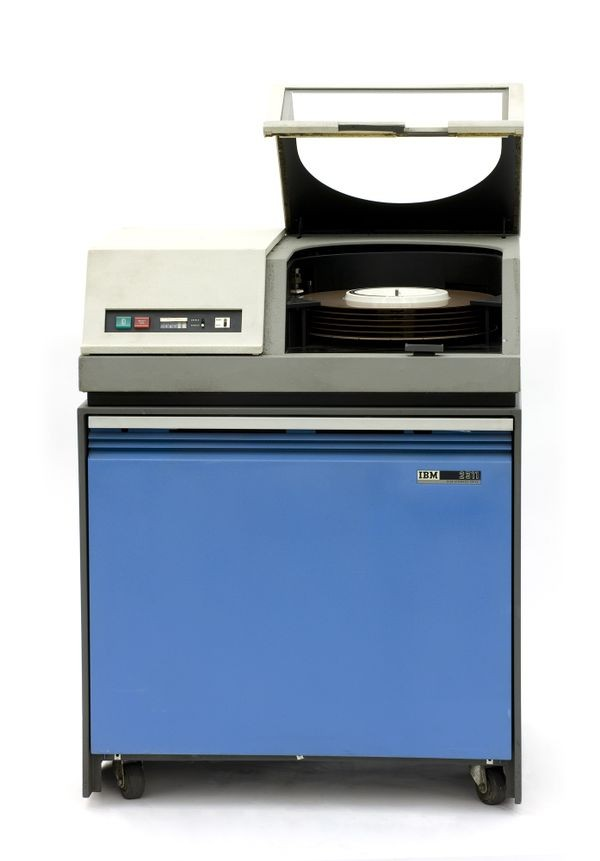
\includegraphics[width=0.5\textwidth,height=\textheight,keepaspectratio]{resources/made/ibmdisk_2311.png}
                    \caption[]{IBM 2311 disk drive}
                \end{figure}
            \end{block}
        \end{column}
    \end{columns}

    \framebreak

    \begin{columns}
        \begin{column}{0.7\textwidth}
            \begin{block}{}
                \blockquote[Bayer and McCreight]{%
                    (\ldots) actual experiments show that it is possible 
                    to maintain an index of size 15.000 with an average of 9 retrievals, 
                    insertions, and deletions per second in real time on an IBM 360/44 
                    with a 2311 disc as backup store. (\ldots) it should be possible 
                    to main tain all index of size 1'500.000 with at least two transactions 
                    per second.}
            \end{block}
            \begin{block}{}
                \blockquote[Bayer]{%
                    I am occasionally asked what the B in B-Tree means. (\ldots)
                    We wanted the name to be short, quick to type, easy to remember.
                    It honored our employer, Boeing Airplane Company, but we wouldn't have to request permission to use the name.
                    It suggested Balance. Rudolf Bayer was the senior researcher of the two of us. (\ldots)
                    I don't recall one meaning standing out above the others that day. 
                    Rudolf is fond of saying that the more you think about what the B could mean, the more you learn about B-Trees, and that is good.
                }
            \end{block}
        \end{column}
        \begin{column}{0.3\textwidth}
            \begin{block}{}
                \begin{figure}
                    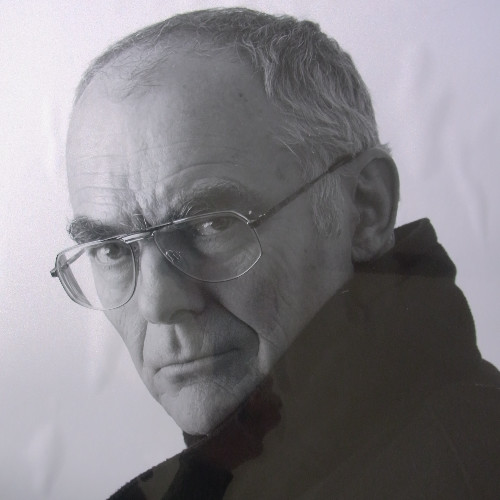
\includegraphics[height=0.3\textheight]{resources/made/r_bayer.png}
                    \caption[]{Rudolf Bayer}
                \end{figure}
                \begin{figure}
                    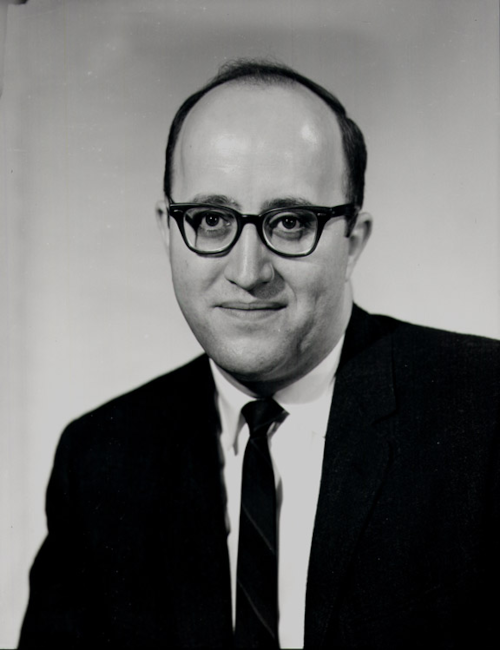
\includegraphics[height=0.35\textheight]{resources/made/McCreight.png}
                    \caption[]{Edward McCreight}
                \end{figure}
            \end{block}
        \end{column}
    \end{columns}
\end{frame}
